\documentclass[10pt,twocolumn,letterpaper]{article}

\usepackage{cvpr}
\usepackage{times}
\usepackage{epsfig}
\usepackage{graphicx}
\usepackage{amsmath}
\usepackage{amssymb}

% Include other packages here, before hyperref.

% If you comment hyperref and then uncomment it, you should delete
% egpaper.aux before re-running latex.  (Or just hit 'q' on the first latex
% run, let it finish, and you should be clear).
\usepackage[pagebackref=true,breaklinks=true,letterpaper=true,colorlinks,bookmarks=false]{hyperref}

% \cvprfinalcopy % *** Uncomment this line for the final submission

\def\cvprPaperID{2254} % *** Enter the CVPR Paper ID here
\def\httilde{\mbox{\tt\raisebox{-.5ex}{\symbol{126}}}}

% Pages are numbered in submission mode, and unnumbered in camera-ready
\ifcvprfinal\pagestyle{empty}\fi
\begin{document}

%%%%%%%%% TITLE
\title{Coupling Uncertain Active Constellation Models with \\
Cascaded Forest Predictors for Sematic Segmentation \\ -- Supplement --}

\author{First Author\\
Institution1\\
Institution1 address\\
{\tt\small firstauthor@i1.org}
% For a paper whose authors are all at the same institution,
% omit the following lines up until the closing ``}''.
% Additional authors and addresses can be added with ``\and'',
% just like the second author.
% To save space, use either the email address or home page, not both
\and
Second Author\\
Institution2\\
First line of institution2 address\\
{\tt\small secondauthor@i2.org}
}

\maketitle
%\thispagestyle{empty}

%%%%%%%%% ABSTRACT
%\begin{abstract}
We will include Figures~\ref{fig:output-over-levels}~and~\ref{fig:var-importance} of the supplementary material into the paper. 

%\end{abstract}

\begin{figure*}[t]
\begin{center}
%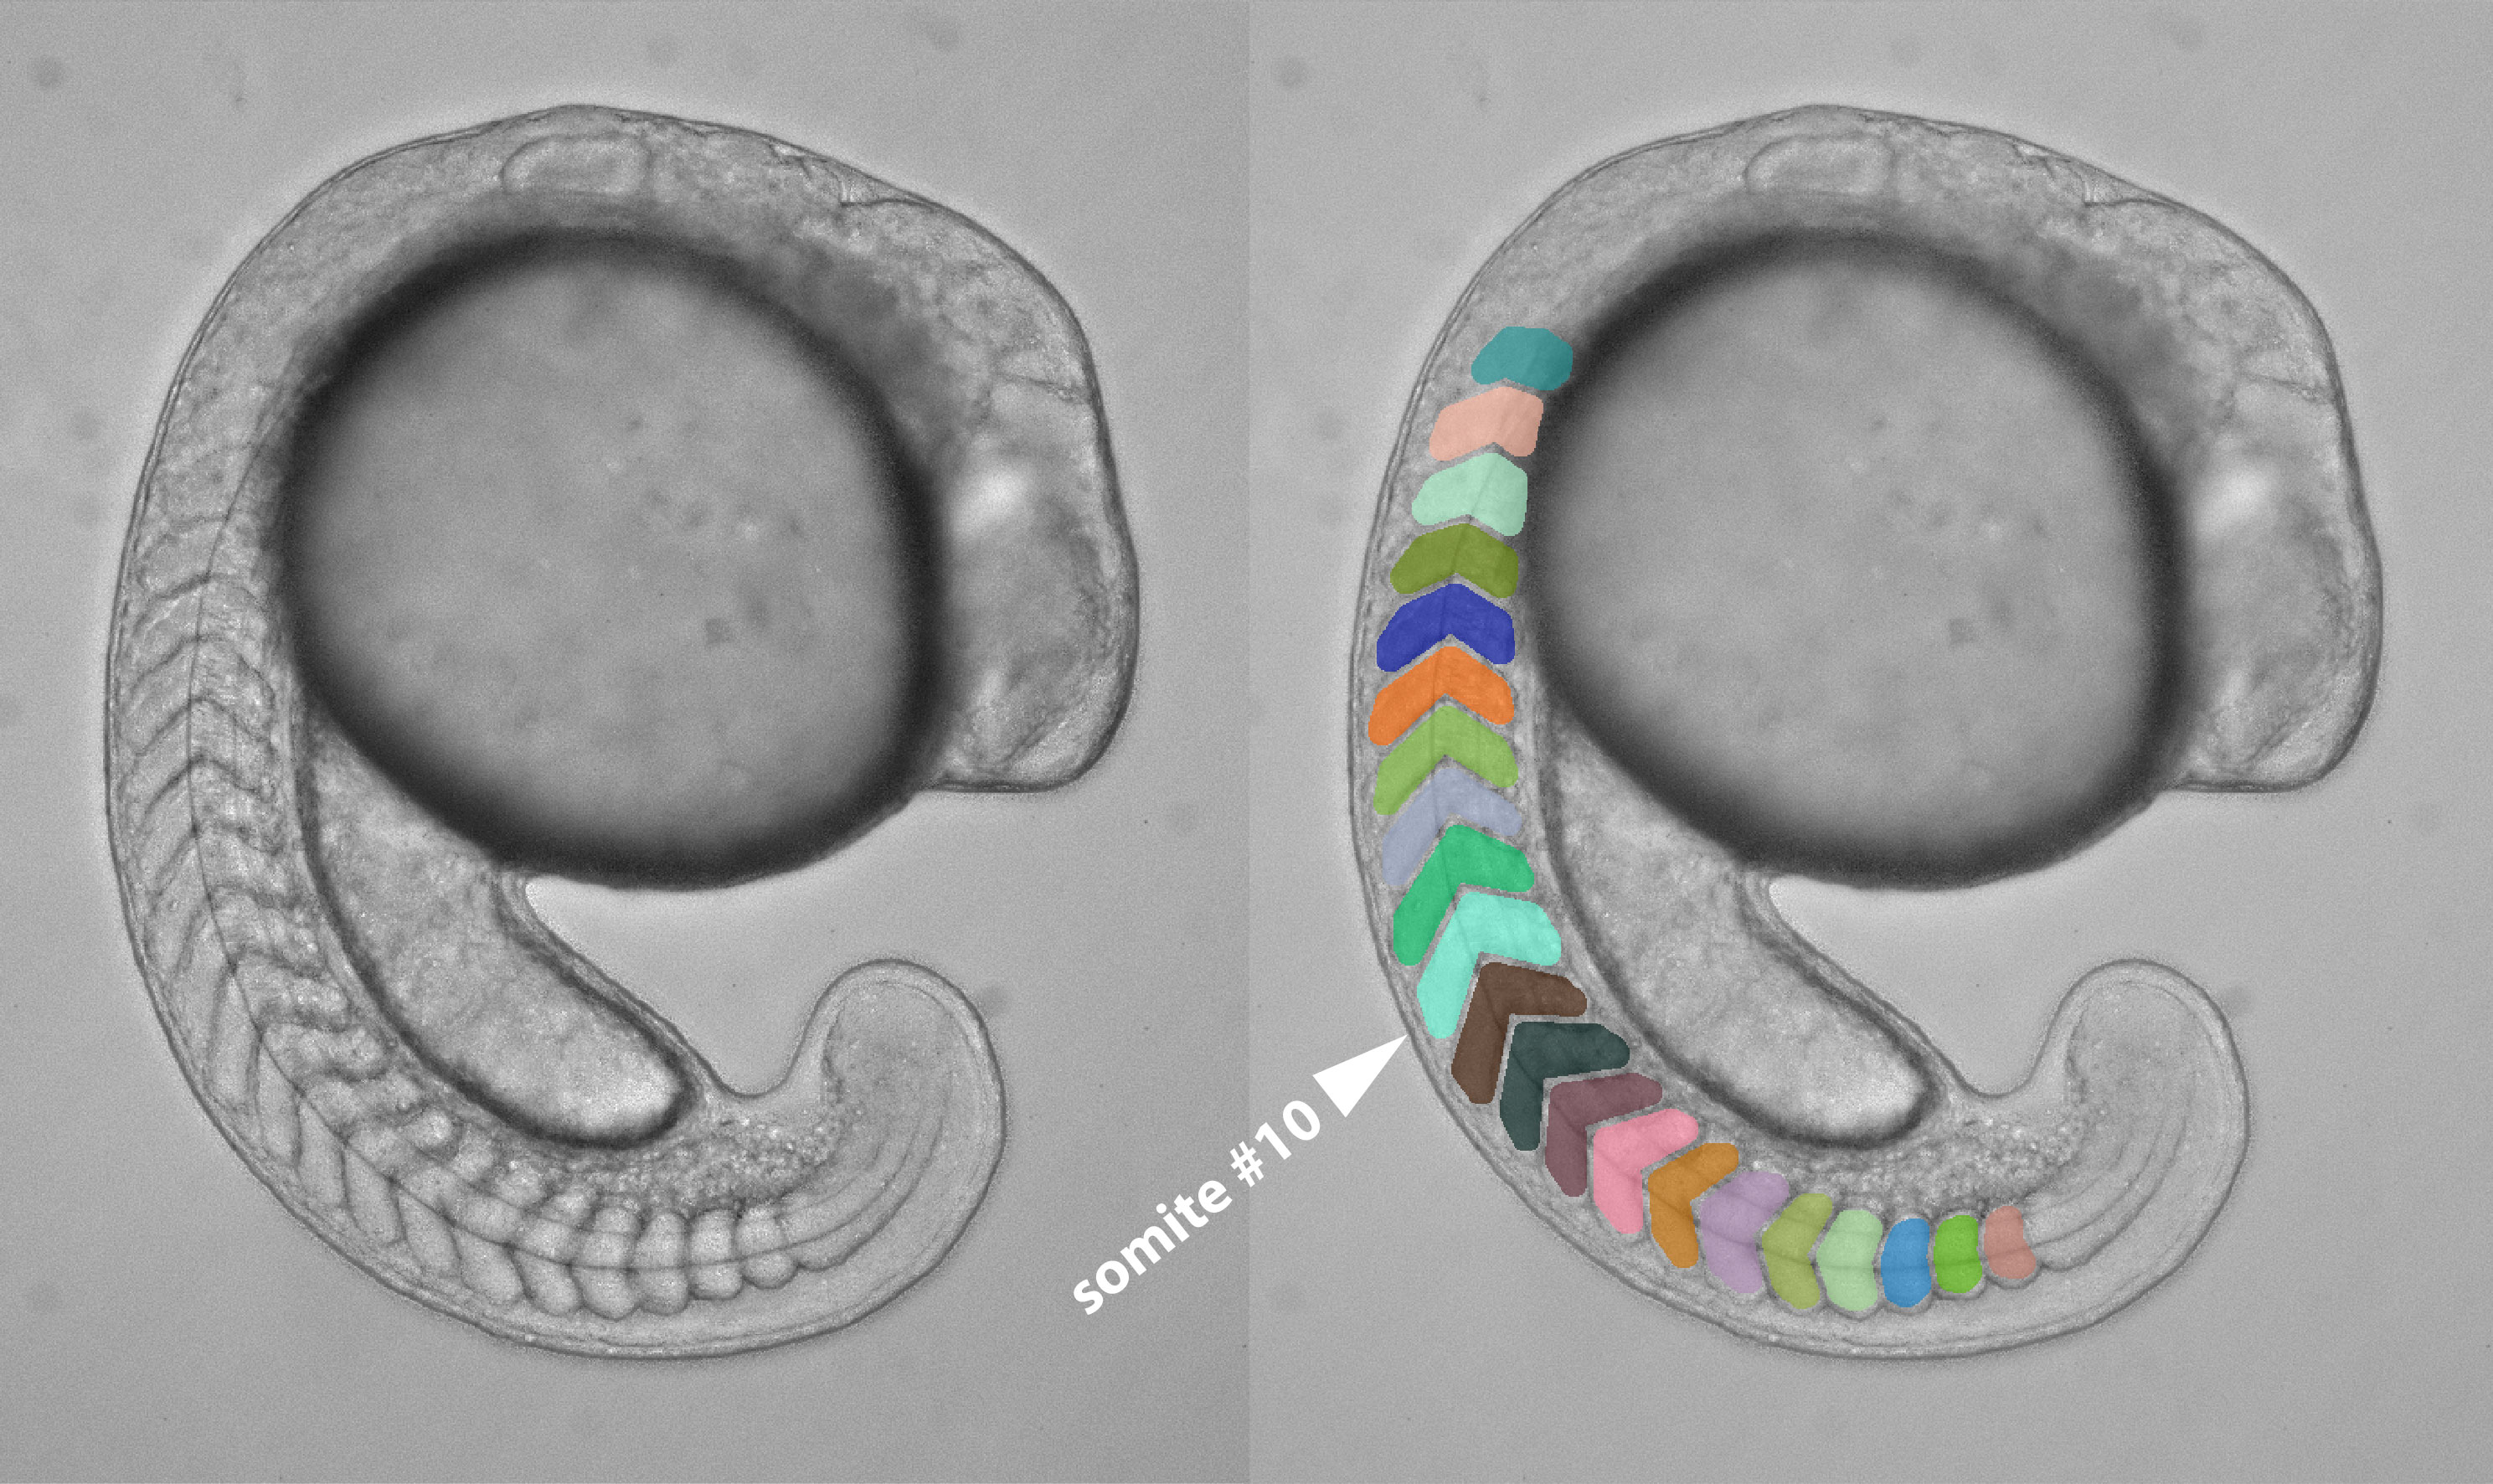
\includegraphics[width=\columnwidth]{TopRight.jpg} 
\caption{Output and smoothed output over levels }
\label{fig:output-over-levels}
\end{center}
\end{figure*}

\begin{figure*}[t]
\begin{center}
%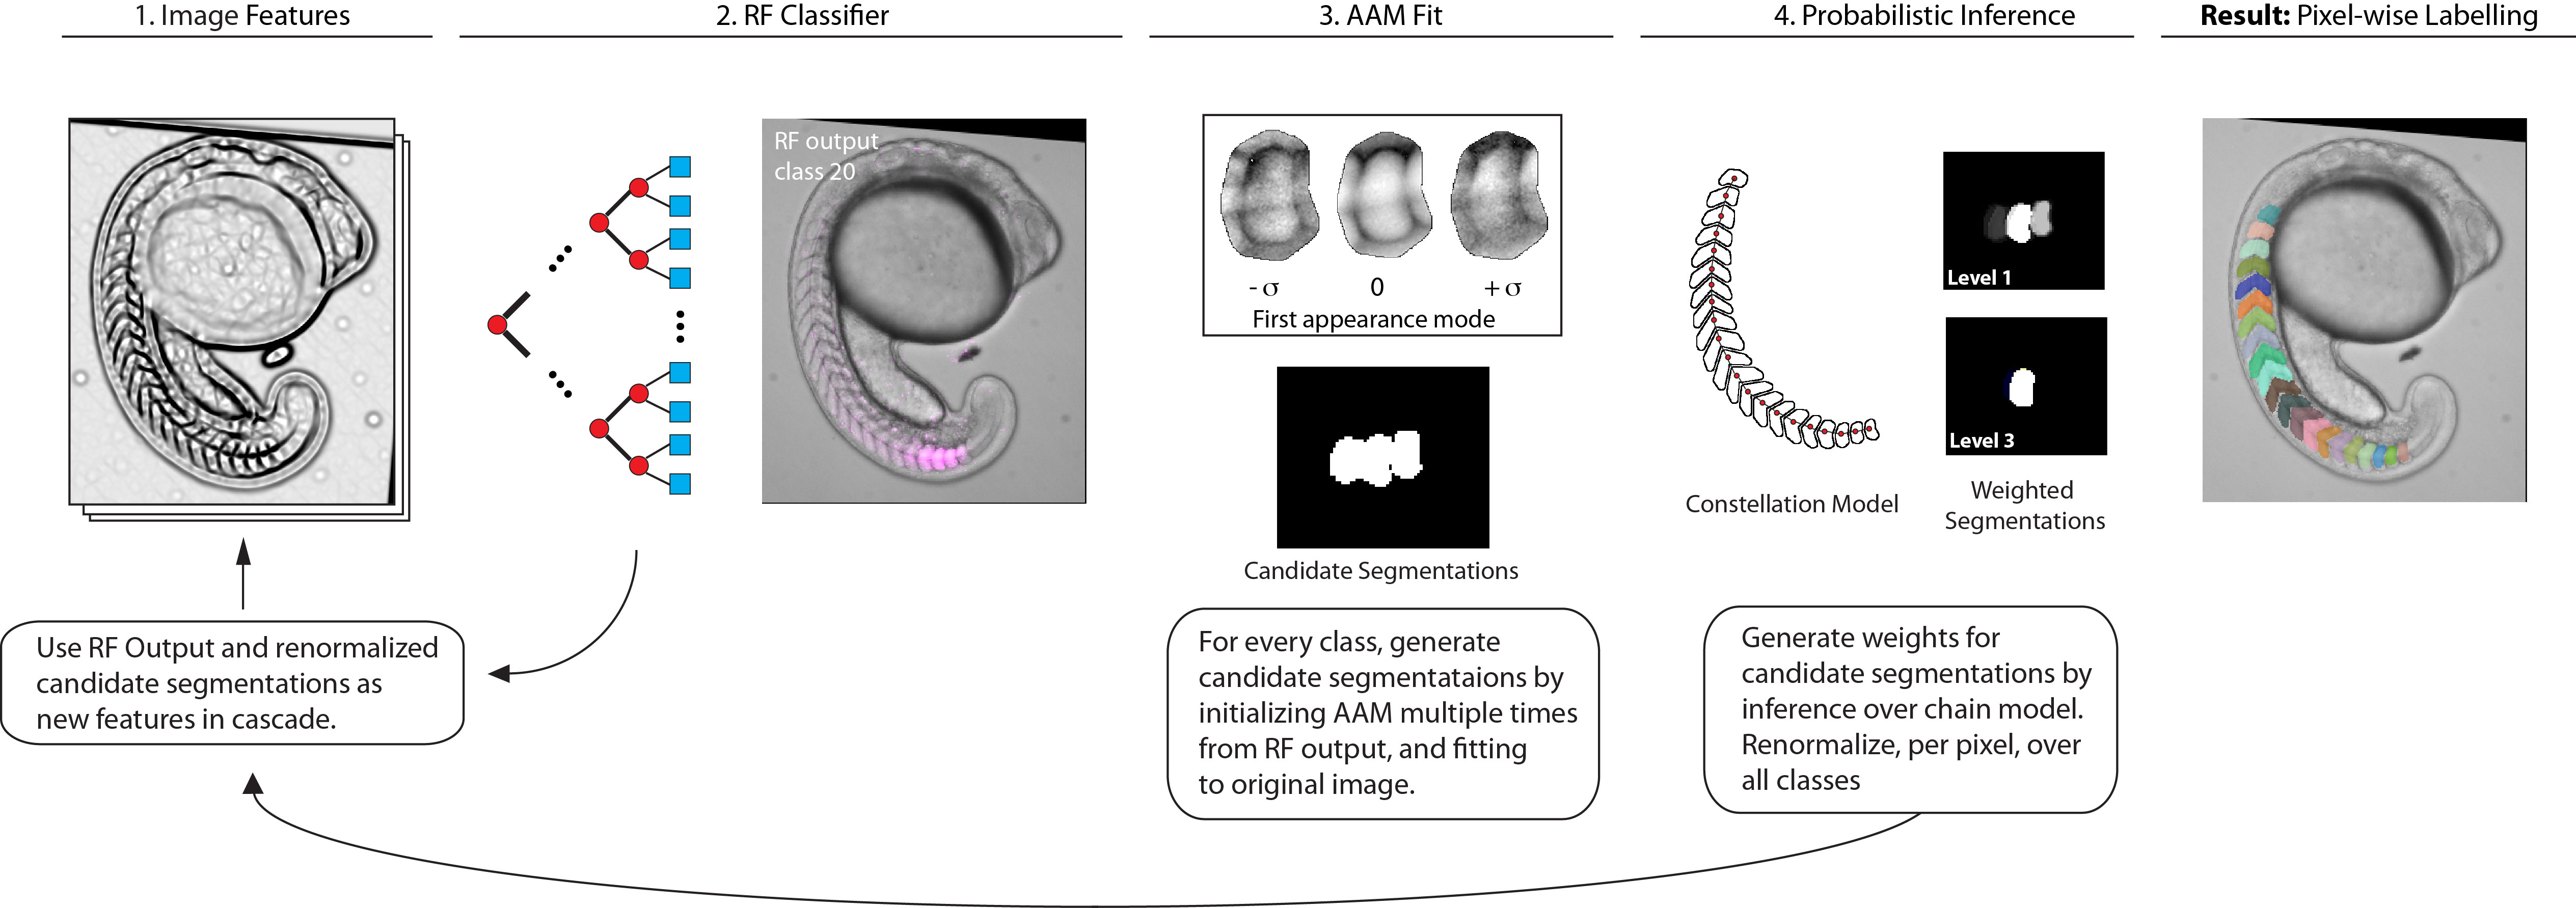
\includegraphics[width=\textwidth]{pipelineBIG2.jpg} 
\caption{Variable Importance.}
\label{fig:var-importance}
\end{center}
\end{figure*}

\begin{figure*}[t]
\begin{center}
%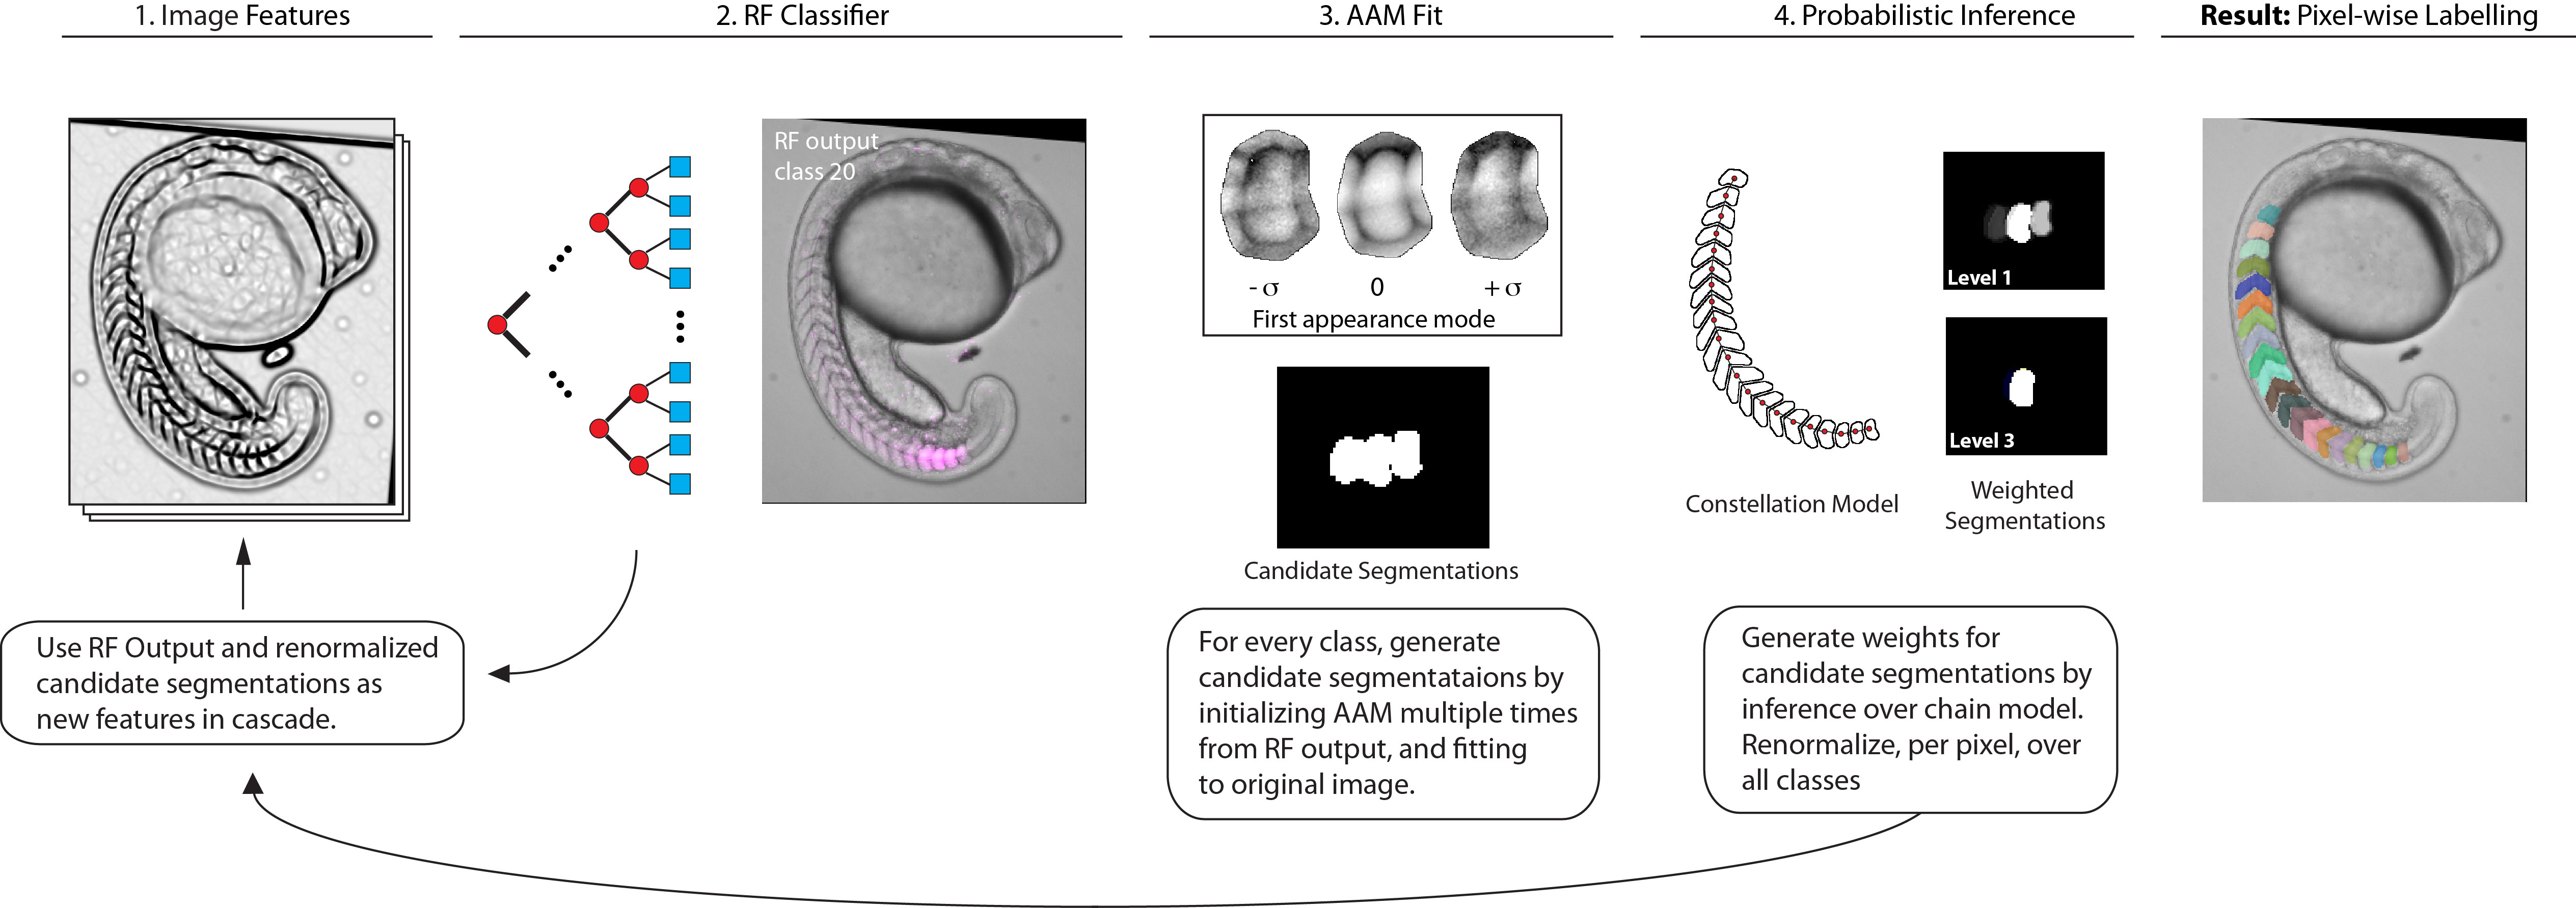
\includegraphics[width=\textwidth]{pipelineBIG2.jpg} 
\caption{Individual methods as box plots with parallel coordinates.}
\label{fig:pcp-plots}
\end{center}
\end{figure*}


\end{document}
